\documentclass[11pt]{article}
\usepackage[toc,page]{appendix}
\usepackage{amsmath, amssymb}
\usepackage[utf8]{inputenc}
\usepackage[T1]{fontenc}
\usepackage[style=apa,backend=biber]{biblatex}
%\usepackage{biblatex}
\addbibresource{references.bib}
\usepackage{graphicx}
\usepackage{tikz}
\usetikzlibrary{automata,positioning,shapes.geometric, arrows.meta, fit, backgrounds, calc, chains}
\graphicspath{./images/Easy_Pictures/SMR_MULT_Repackaging}%\usepackage{kpfonts}
\usepackage{float}
\usepackage[margin=1in]{geometry}
\usepackage{cancel}
\usepackage{epsfig}
\usepackage{tikz-3dplot}
\usepackage{darkmode}
\usepackage{dirtytalk}
\usepackage{longtable,booktabs,array}
\usepackage{calc} % for calculating minipage widths
\usepackage[utf8]{inputenc}
\usepackage[T1]{fontenc}
\usepackage{xcolor}
\usepackage{listings}


\usepackage{etoolbox}
\usepackage{hyperref}
\hypersetup{
 colorlinks=true,
 linkcolor=blue,
 filecolor=magenta, 
 urlcolor=cyan,
 pdftitle={Hermeneutic Calculator},
 citecolor=blue,
 }


\urlstyle{same}

\lstdefinestyle{htmlStyle}{
 language=HTML,
 basicstyle=\ttfamily\small,
 keywordstyle=\color{blue}\bfseries,
 commentstyle=\color{gray}\itshape,
 stringstyle=\color{red},
 breaklines=true,
 frame=single,
 numbers=left,
 numberstyle=\tiny\color{gray},
 columns=fullflexible,
}
\lstdefinelanguage{HTML}{
 keywords={<!DOCTYPE, html, head, title, body, h1, h2, h3, p, div, span, a, img, ul, li, table, tr, td, th, style, link, script},
 sensitive=true,
 comment=[l]{//},
 morecomment=[s]{/*}{*/},
 morestring=[b]',
 morestring=[b]"
}
\lstset{style=htmlstyle, language=html}
% Updated to explicitly pass the language option
%\lstinputlisting[style=htmlstyle, language=html]{./html/example.html}
%\usepackage{tocloft}

% Optional: define some custom colors
\definecolor{sliceRed}{RGB}{225,224,91} % matching "varyellow" from your code
\definecolor{linkYellow}{RGB}{255,215,0} % a golden yellow
\tdplotsetmaincoords{70}{110}

\title{Subtraction Strategies: Sliding to Make Bases}
\author{Compiled by: Theodore M. Savich}


\begin{document}
\maketitle
\subsection*{Transcript}
 Strategy descriptions and examples adapted from \textcite{HackenbergCourseNotes}. This is not based on a CGI video. I fake a student example. 

\begin{itemize}
\item Teacher: John had 73 pieces of halloween candy. He gave 47 pieces to his friend. How many pieces of candy does John have left?
\item Student: I can pretend I gave away 50 pieces and also pretend I had three more than I did. So that's like 76-50, which is 26. 
\end{itemize}

\noindent \textbf{Notation Representing Rita's Solution:}
\begin{align*}
    73 - 47 &= \Box\\
    73+3 &= 76\\
    47+3 &= 50\\
    73 - 47 &= 76 - 50\\
    &= 26
\end{align*}

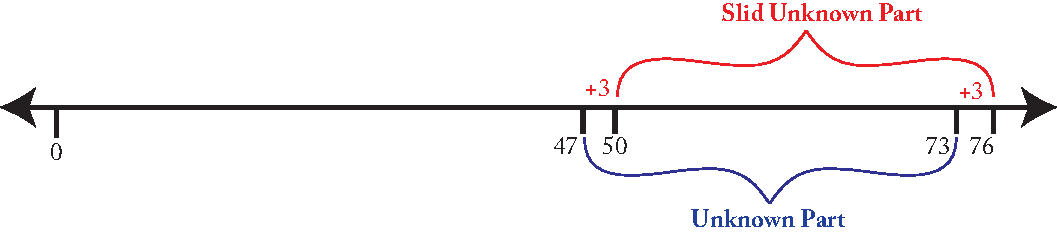
\includegraphics[width=.8\textwidth]{images/Easy_Pictures/SAR_SUB_Sliding/PDF/SAR_SUB_Sliding.pdf}

\noindent In the sliding strategy, you adjust both the number you’re subtracting from (the whole) and the number being subtracted (the part) by the same amount. The goal is to shift the subtrahend into a `friendly' number (usually a multiple of a base). By doing this, the difference between the adjusted values remains identical to the original difference, simplifying the subtraction process.


\subsubsection*{Description of Strategy}
\begin{itemize}
    \item \textbf{Objective:} Adjust both the minuend (known whole) and subtrahend (known part) by the same amount to make the subtraction easier, keeping the difference the same.
\end{itemize}

\subsubsection*{Automaton Type}
\textbf{Finite State Automaton (FSA)}: Adjustments are made consistently and can be tracked without additional memory.

\subsubsection*{Formal Description of the Automaton}

We define the automaton as the tuple
\[
M = (Q,\,\Sigma,\,\delta,\,q_{0/accept},\,F)
\]
where:
\begin{itemize}
    \item \(Q = \{q_{0/accept},\, q_1,\, q_2,\, q_3\}\) is the set of states.
    \item \(\Sigma = \{0,1,2,3,4,5,6,7,8,9\}\) is the input alphabet (representing the digits of the minuend \(M\) and subtrahend \(S\)).
    \item \(q_{0/accept}\) is the start state, which is also the accept state.
    \item \(F = \{q_{0/accept}\}\) is the set of accepting states.
\end{itemize}

The transition function \(\delta\) is defined as follows:
\begin{enumerate}
    \item \(\delta(q_{0/accept},\, \text{``}M,S\text{''}) = q_1\) \quad (Calculate the adjustment needed to make the subtrahend a base multiple.)
    \item \(\delta(q_1,\, \varepsilon) = q_2\) \quad (Adjust both the minuend and subtrahend by the same amount.)
    \item \(\delta(q_2,\, \varepsilon) = q_3\) \quad (Perform the subtraction on the adjusted numbers.)
    \item \(\delta(q_3,\, \varepsilon) = q_{0/accept}\) \quad (Output the final difference.)
\end{enumerate}

\subsubsection*{Automaton Diagram for Sliding to Make Bases}

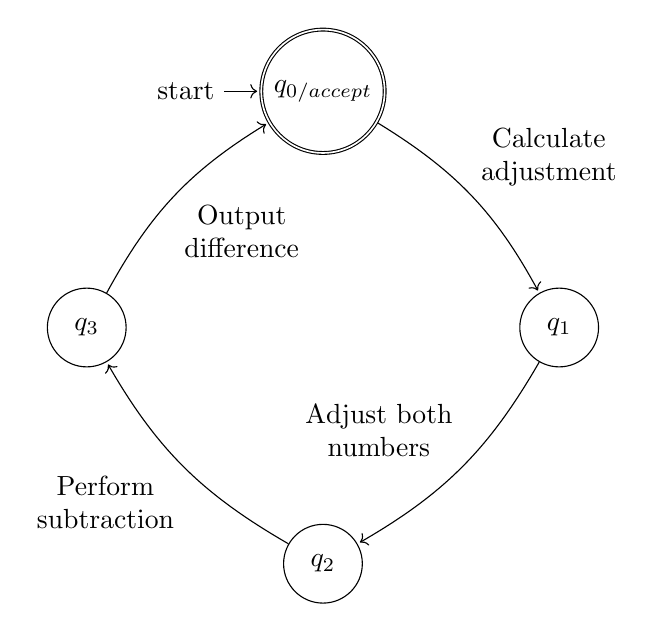
\begin{tikzpicture}[
    shorten >=1pt,
    auto,
    node distance=3cm,
    every state/.style={minimum size=1cm}
]
    % Arrange 4 states on a circle.
    \node[state, initial, accepting] (q0) at (90:3cm) {$q_{0/accept}$};
    \node[state] (q1) at (0:3cm) {$q_1$};
    \node[state] (q2) at (270:3cm) {$q_2$};
    \node[state] (q3) at (180:3cm) {$q_3$};

    \path[->]
        (q0) edge[bend left=15] node[above right, align=center] {Calculate\\adjustment} (q1)
        (q1) edge[bend left=15] node[above left, align=center] {Adjust both\\numbers} (q2)
        (q2) edge[bend left=15] node[below left, align=center] {Perform\\subtraction} (q3)
        (q3) edge[bend left=15] node[below right, align=center] {Output\\difference} (q0);
\end{tikzpicture}

\clearpage
\subsubsection*{HTML Implementation}
\lstinputlisting[style=htmlStyle, language=html]{./new_html/SAR_SUB_Sliding.html}

\printbibliography
\end{document}